\section{计算机系统概述}

\subsection{操作系统的基本概念}
操作系统(Operating System, OS)是计算机系统中最基本的系统软件。

\subsubsection{特征}
\begin{enumerate}
    \item 并发(Concurrence): 指两个或多个事件在同一时间间隔内发生
    \subitem 与之相关, 并行是指两个或多个事件在同一时刻发生
    \item 共享(Sharing)
    \item 虚拟(Virtual)
    \item 异步(Asynchronism): 多道程序环境允许多个程序并发执行. 
\end{enumerate}

\subsection{操作系统发展历程}
\begin{enumerate}
    \item 单道批处理系统(Batch Processing)
    \item 多道批处理系统(Multiprogramming Batch Processing System): 一段时间内内存中同时存在多个进程, 即并发任务. 
    \item 分时操作系统(Time Sharing Systems): 分时系统通过频繁地在多个进程间切换来近似实现并行
\end{enumerate}

\subsection{操作系统运行}

\subsubsection{特权模式(Privileged Mode)}
将CPU的运行模式划分为用户态(User Mode)和内核态(Kernel Mode). 特权指令(privileged instruction), 是指不允许用户直接使用的指令. 模式的切换是通过 trap 实现的. 

\subsubsection{计时器(timer)}
通过时钟中断的管理, 可以实现进程的切换. 

\subsubsection{中断(Interrupt)}
\begin{itemize}
    \item 中断(Interruption): 指来自CPU执行指令外部的事件, 如信息, 设备的 I/O
    \item 异常(Exception): 指来自CPU执行指令内部的事件
\end{itemize}

\begin{figure}[H]
    \centering
    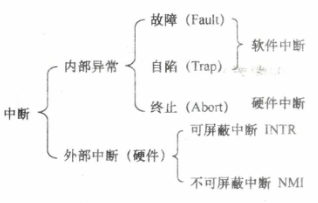
\includegraphics[width=0.618\linewidth]{pic/OS-CheatSheet/内中断和外中断的联系与区别}
    \caption{内中断和外中断的联系与区别}
\end{figure}


\subsubsection{系统调用(System Call)}
用户在程序中调用操作系统所提供的一些子功能, 系统调用可视为特殊
的公共子程序. 

\subsection{操作系统结构}
\begin{enumerate}
    \item 分层法
    \item 模块化
    \item 宏内核
    \item 微内核
    \item 外核
\end{enumerate}

\subsection{引导(bootstrap)}
在计算机刚刚启动, 操作系统还未开始运行之前, 需要开机后的第一个程序——引导加载器(bootstrap loader)来一步一步地初始化操作系统。对大多数操作系统来说, bootstrap 都会被存储在 ROM 中, 并且需要在一个已知的位置. 

BIOS :基本I/O系统